\documentclass[12pt]{article}
\usepackage{setspace}
\setlength{\parindent}{4em}
\usepackage{fancyvrb}
\usepackage{graphicx}
\usepackage{geometry}
\renewcommand\thesection{\arabic{section}}
\renewcommand\thesubsection{\thesection.\arabic{subsection}}
\geometry{letterpaper, portrait, margin=1in}

%%%Title Page%%%
\title{\vspace{3cm}Lab 05\bigbreak Designing the Controller of the CPU}
\author{
{\normalsize
\begin{tabular}{l r r}
 & \textbf{Ryan Cruz} & \textbf{Zachary Davis}\\
\textbf{Category} & ryan.cruz25@uga.edu & zachdav@uga.edu\\
\hline
Pre-lab 						  & 50 & 50\\
In-lab Module \& Testbench Design & 50 & 50\\
In-lab Testbench Sim. \& Analysis & 50 & 50\\
In-lab FPGA Synthesis \& Analysis & 50 & 50\\
Lab Report Writing 				  & 50 & 50\\
\end{tabular}
}}
%%%%%%%%%%%%%%%%%

\begin{document}
\maketitle
\newpage
\setstretch{2.5} % for custom spacing
\tableofcontents
\setstretch{1} % for custom spacing
\newpage

\section{Lab Purpose} \vspace{-.7cm} \line(1,0){470}
	\paragraph{} 		
		
\section{Implementation Details} \vspace{-.7cm} \line(1,0){470}
		\subsection{Prelab}

		\begin{figure}[h]
		\centering
			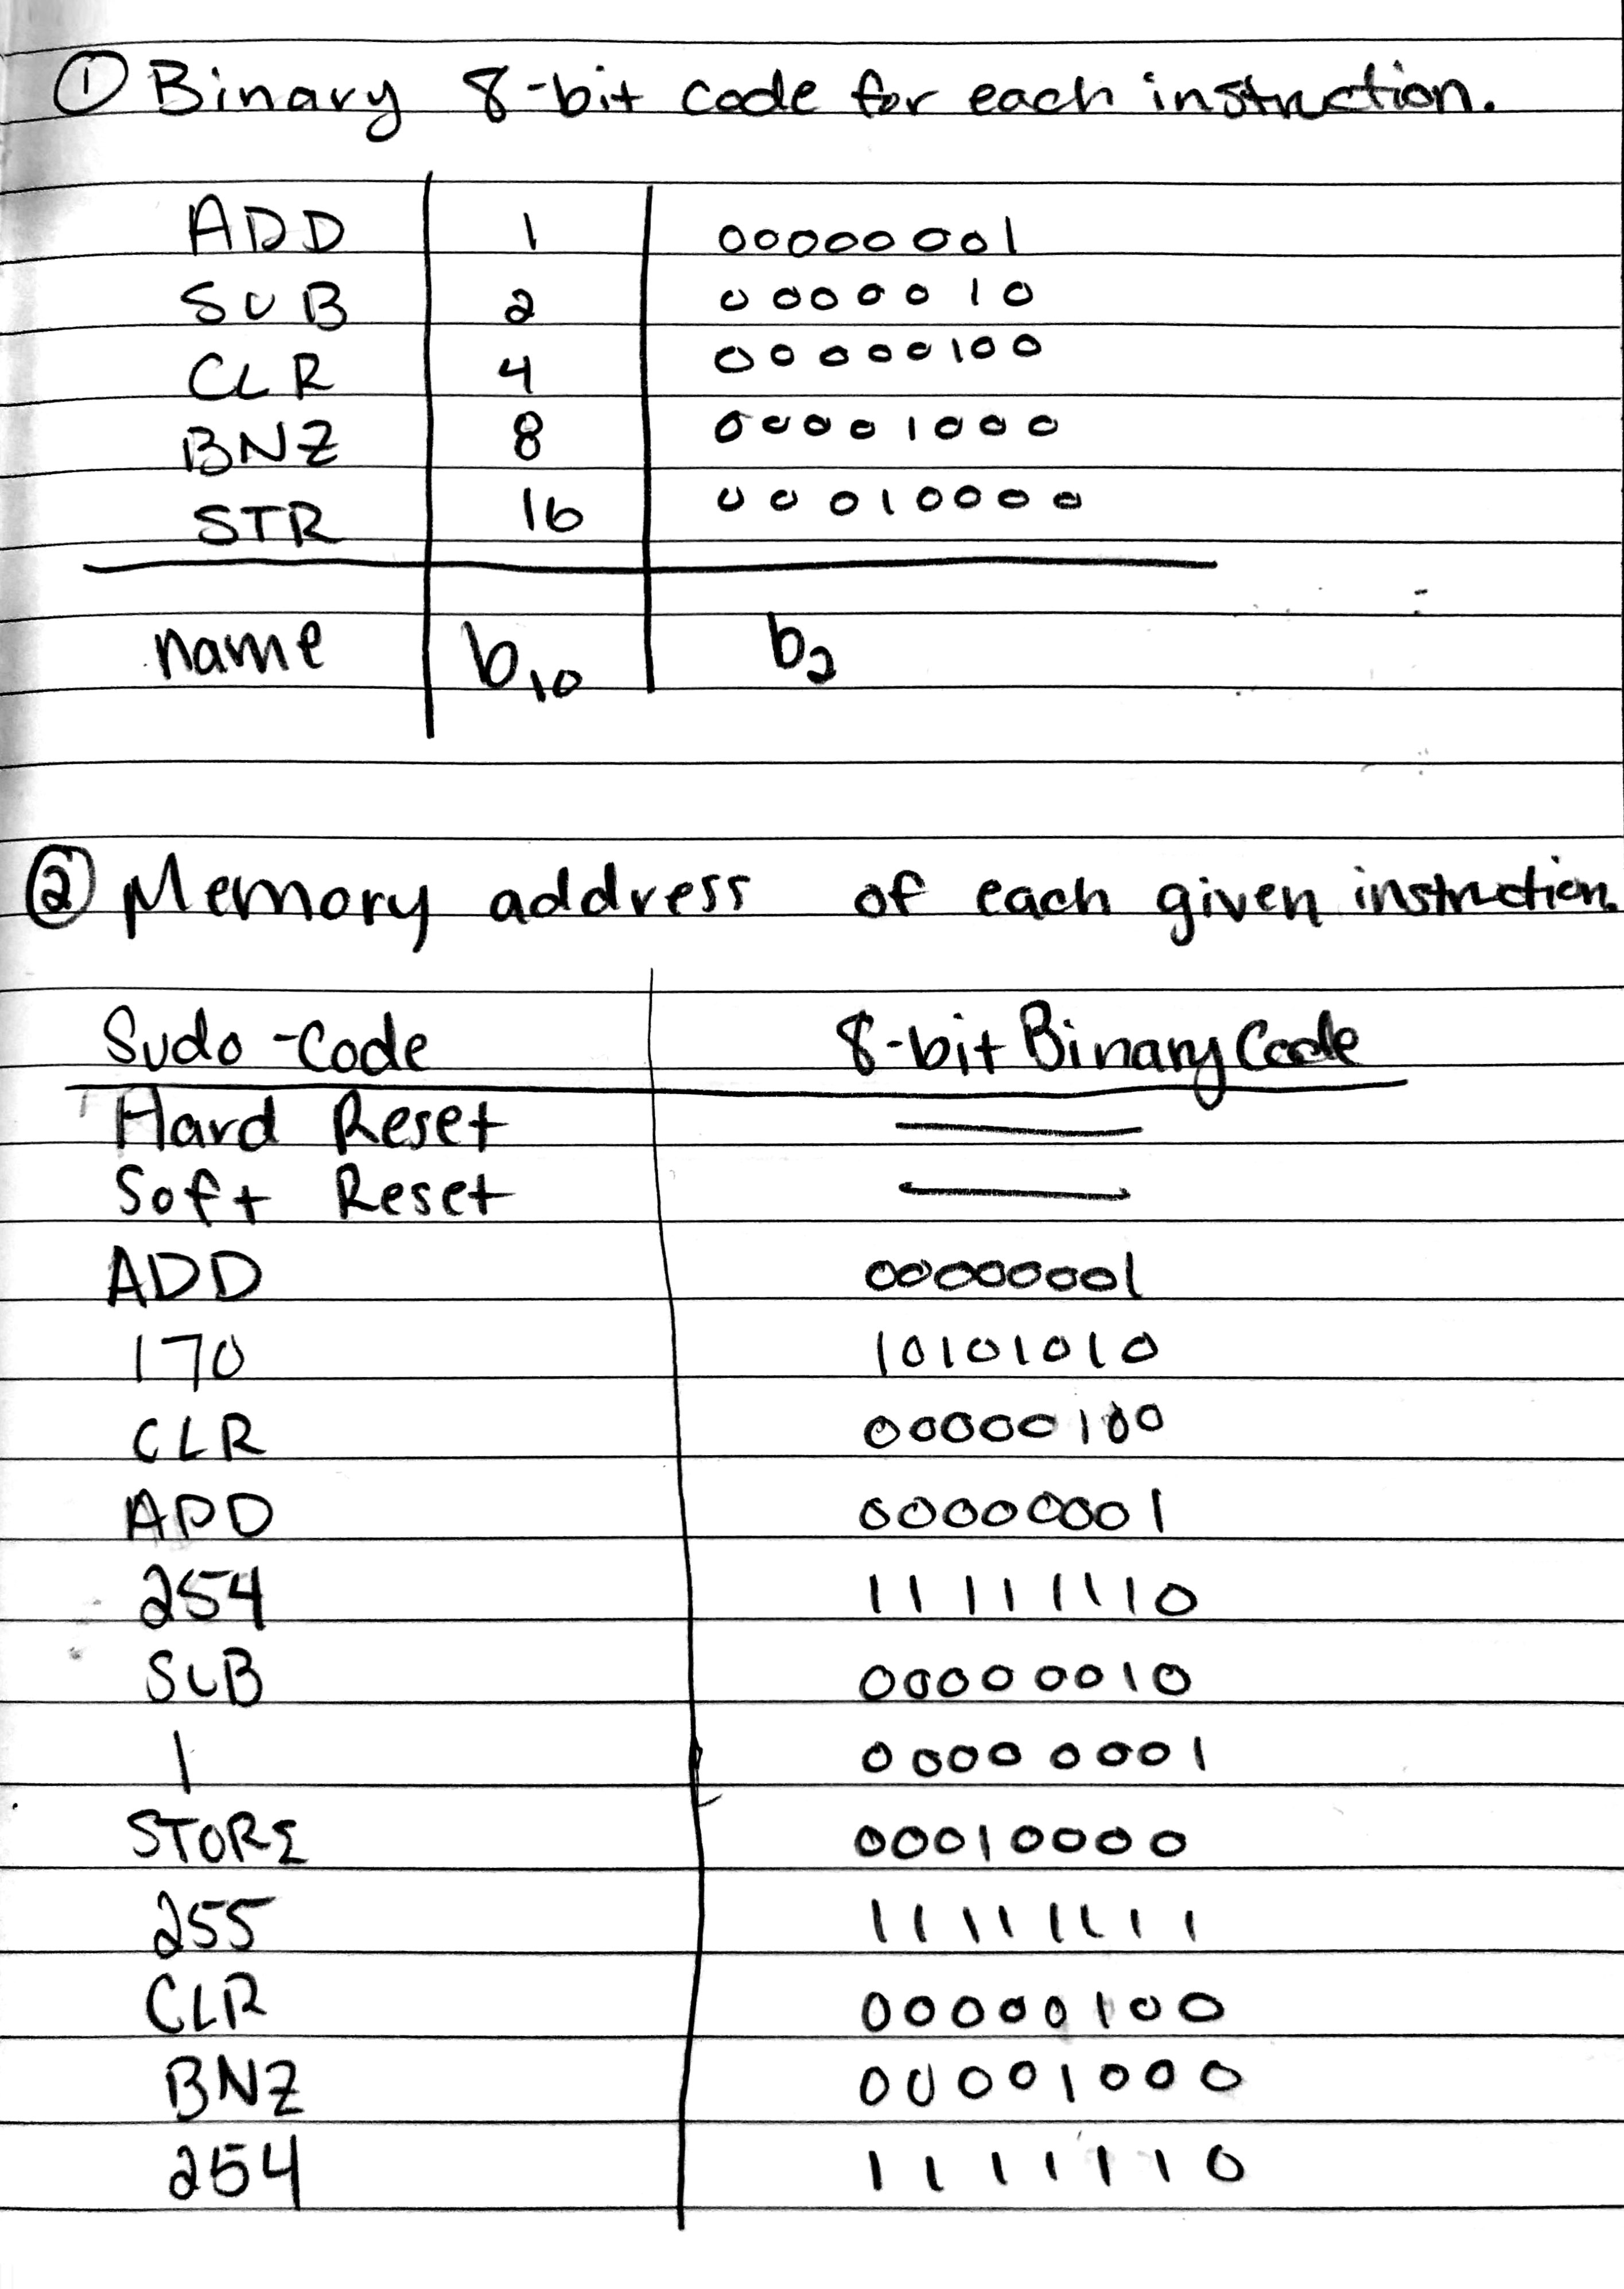
\includegraphics[scale=.11]{Prelab.jpg}
			\caption{The Binary 8-bit code for each instruction, as well as the memory addresses for each given instruction.}
		\end{figure}

		

	\subsection{Circuit Implementation in Schematic Editor}
		\paragraph*{}
			
		\begin{figure}[h]
			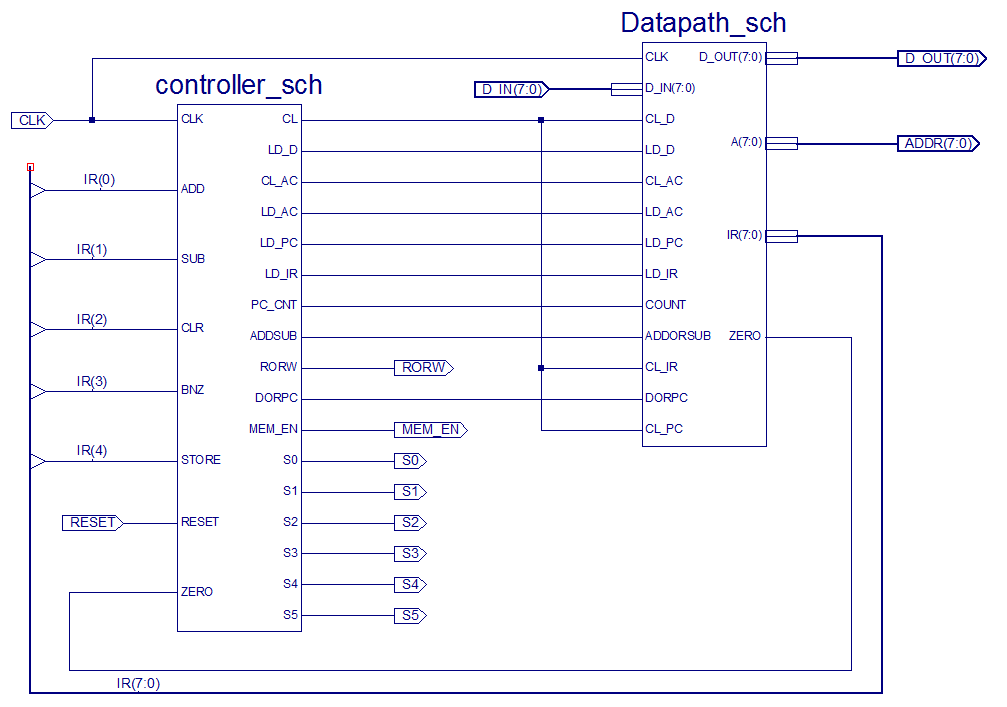
\includegraphics[scale=.6]{toy_sch.PNG}
			\caption{}
		\end{figure}
		
		\newpage
	\subsection{Simulation}
		

		
		\begin{Verbatim}[frame=single, fontsize= \small]

	
		\end{Verbatim}
		
			
\section{Experimental Results}\vspace{-.7cm} \line(1,0){470}

\begin{figure}[h]
    \centering
	%\includegraphics[scale=.48]{}
	\caption{}
\end{figure}

\begin{figure}[h]
    \centering
	%\includegraphics[scale=.33]{}
	\caption{}
\end{figure}


	\newpage
\section{Significance} \vspace{-.7cm} \line(1,0){470}
	\paragraph{} 


 \section{Comments/Suggestions}\vspace{-.7cm} \line(1,0){470}
 	\paragraph{} 
		
\end{document}


